\documentclass{standalone}
\usepackage{pgfplots}
\begin{document}
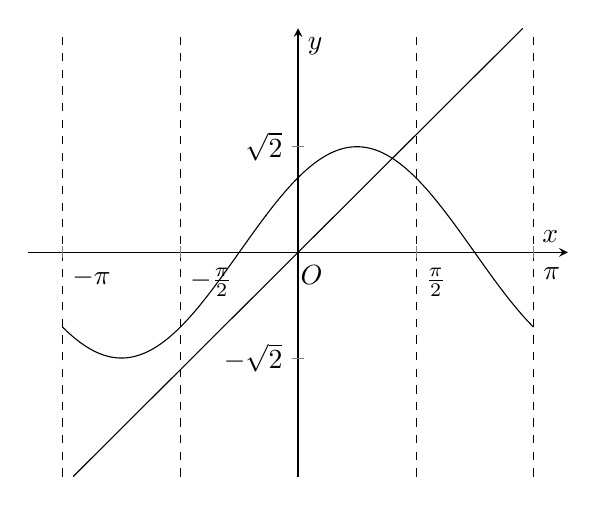
\begin{tikzpicture}
\begin{axis}
[
ymin=-3,ymax=3,
xmin=-3.6,xmax=3.6,
xtick=\empty,
ytick=\empty,
extra x ticks={-3.14159, -1.5708, 1.5708, 3.14159},
extra x tick labels={$-\pi$, $-\frac{\pi}{2}$, $\frac{\pi}{2}$, $\pi$},
extra y ticks={-1.41421, 1.41421},
extra y tick labels={$-\sqrt{2}$, $\sqrt{2}$},
every extra x tick/.style={
    xticklabel style={anchor=north west},
    grid=major,
    major grid style={very thin,dashed,black}
},
axis lines = center,
xlabel=$x$,ylabel=$y$,
samples=200,
]
\addplot [black, domain=-3.14159:3.14159] {sin(deg(x)) + cos(deg(x))};
\addplot [black, domain=-3:3] {x};
\node at (axis cs:0.18, -0.3) {$O$} ;
\end{axis}
\end{tikzpicture}
\end{document}
